\documentclass[conference]{IEEEtran}
\IEEEoverridecommandlockouts

\usepackage{cite}
\usepackage{amsmath,amssymb,amsfonts}
\usepackage{graphicx}
\usepackage{textcomp}
\usepackage{xcolor}
\usepackage{booktabs}
\usepackage{url}
\usepackage{tikz}
\usetikzlibrary{arrows.meta,positioning}

\begin{document}

\title{Multi-Agent Deep Reinforcement Learning with Digital Twin Synchronization for Energy-Efficient Smart City IoT Networks}

\author{
\IEEEauthorblockN{Author Name}
\IEEEauthorblockA{\textit{Department of Computer Science and Engineering} \\
\textit{University Name}\\
City, Country \\
email@example.com}
}

\maketitle

\begin{abstract}
Battery-powered Internet of Things (IoT) devices in smart cities must balance two conflicting goals: transmitting pending sensor data on time and conserving energy to extend device lifetime. This paper presents a framework in which each IoT device is controlled by an independent Deep Q-Network (DQN) agent that learns, from its own battery level and pending-data queue, whether to transmit or to sleep. A digital twin maintains a live virtual replica of every device and is synchronized with the physical layer over the MQTT publish--subscribe protocol. The framework is evaluated in a simulated environment and in an environment whose energy cost is driven by real consumption readings from five households, using 10 random seeds. In both environments, the trained agents retain about 12--14\% more battery than a random policy, at a comparable pending-queue length, and obtain more than three times its return. A hand-designed queue-threshold rule obtains a higher return than the learned agents, which we attribute to the short episodes, in which the battery rarely limits behavior. In a test of the MQTT synchronization over a public broker, all 1000 published device states reached the twin, with a median delay of 0.29~s. A Streamlit dashboard visualizes the twin state and the learning progress in real time.
\end{abstract}

\begin{IEEEkeywords}
Internet of Things, digital twin, multi-agent reinforcement learning, deep Q-network, energy efficiency, smart city, MQTT
\end{IEEEkeywords}

\section{Introduction}
\label{sec:intro}

Smart city deployments rely on large numbers of battery-powered Internet of Things (IoT) devices, such as environmental sensors, smart meters, and traffic monitors, that continuously generate data and report it over wireless links \cite{zanella2014}. Radio transmission is one of the most energy-intensive operations of such a device, so the choice of \emph{when} to transmit and \emph{when} to sleep directly determines its lifetime. Transmitting too eagerly drains the battery, while sleeping too long lets unsent data accumulate and delays reporting. Fixed duty-cycle schedules do not adapt to the changing load and battery state of each device.

Reinforcement learning (RL) is a natural fit for this problem, because an agent can learn a transmit-or-sleep policy directly from interaction, without an explicit model of the device's energy dynamics. Deep Q-Networks (DQN) \cite{mnih2015} extend Q-learning with neural function approximation and work well when the action space is small and discrete, as it is here. In a city-scale deployment, however, each device observes only its own state, so the problem is naturally multi-agent: every device needs its own decision-maker, and a single centralized controller would require continuous state reporting from all devices, which itself costs energy.

A second requirement is visibility. Operators need an up-to-date view of every device's state without querying the devices directly. A digital twin, a virtual replica that mirrors the state of a physical asset \cite{grieves2017}, provides this view. In practice, the physical devices and the twin run on different machines, so the twin must be synchronized over a lightweight messaging protocol. MQTT \cite{mqtt} is a widely used publish--subscribe protocol for exactly this purpose in IoT systems.

This paper combines these ideas in one end-to-end framework: each IoT device is controlled by its own DQN agent that chooses between \emph{sleep} and \emph{send}, and a digital twin keeps a live replica of every device over MQTT. The agents are trained independently.

The main contributions of this work are:
\begin{itemize}
    \item A per-device DQN formulation of the transmit-or-sleep decision, with a reward that favors clearing pending data when the queue grows and conserving energy when it is empty, and penalizes battery depletion.
    \item A digital twin layer that mirrors the state of every device and is synchronized with the physical layer over MQTT, together with a real-time dashboard for monitoring.
    \item An environment whose battery drain is driven by real household energy-consumption readings from five households, in addition to a fully simulated environment.
    \item An experimental comparison over 10 random seeds, in both environments, of the trained agents against random, always-send, always-sleep, and queue-threshold policies, including an honest account of where a simple heuristic outperforms the learned policy.
\end{itemize}

\section{Related Work}
\label{sec:related}

\subsection{Energy-Efficient IoT Operation and Reinforcement Learning}
Reducing the energy cost of radio communication has long been studied in wireless sensor networks. Classical approaches rely on fixed or schedule-based duty cycling, in which nodes alternate between active and sleep periods, as in S-MAC \cite{ye2002smac}. These schemes are simple, but their schedules are set in advance and do not react to the instantaneous battery level or data backlog of a node. Reinforcement learning has therefore been applied to communication and networking problems as an adaptive alternative; a comprehensive survey is given in \cite{luong2019}. Reinforcement learning has also been used to control the channel access of battery-limited IoT devices, for example in \cite{chu2019}. Our work follows this line, but formulates the problem at the level of a single device that chooses between sleeping and transmitting based on its own battery and queue state.

\subsection{Multi-Agent Reinforcement Learning}
When several decision-makers act in the same environment, the problem becomes a multi-agent reinforcement learning (MARL) problem; an overview of the theory and algorithms is given in \cite{zhang2021marl}. The simplest approach is independent learning, where each agent applies single-agent Q-learning and treats the others as part of the environment \cite{tan1993}. In this work we adopt independent DQN agents \cite{mnih2015}, one per device. This choice keeps each agent lightweight and requires no communication between devices, at the cost of ignoring interactions between them.

\subsection{Digital Twins for IoT and Networks}
A digital twin is a virtual representation of a physical asset that is kept consistent with it through data exchange \cite{grieves2017}. Surveys describe the enabling technologies and open challenges of digital twins \cite{fuller2020} and their use in industry \cite{tao2019}. Digital twins have also been combined with learning-based control in wireless and edge networks \cite{lu2021}. In most such systems the twin is used for monitoring, simulation, or offline training. In our framework the twin is a live mirror of every device, synchronized over MQTT \cite{mqtt}, which separates the monitoring layer from the physical devices.

\section{System Architecture}
\label{sec:system}

The framework has four layers, shown in Fig.~\ref{fig:arch}: the IoT device layer, the agent layer, the digital twin layer, and a monitoring dashboard. Each device is controlled by its own agent. Device states are published through an MQTT broker, and the digital twin subscribes to them and maintains a live replica of every device.

\begin{figure*}[t]
\centering
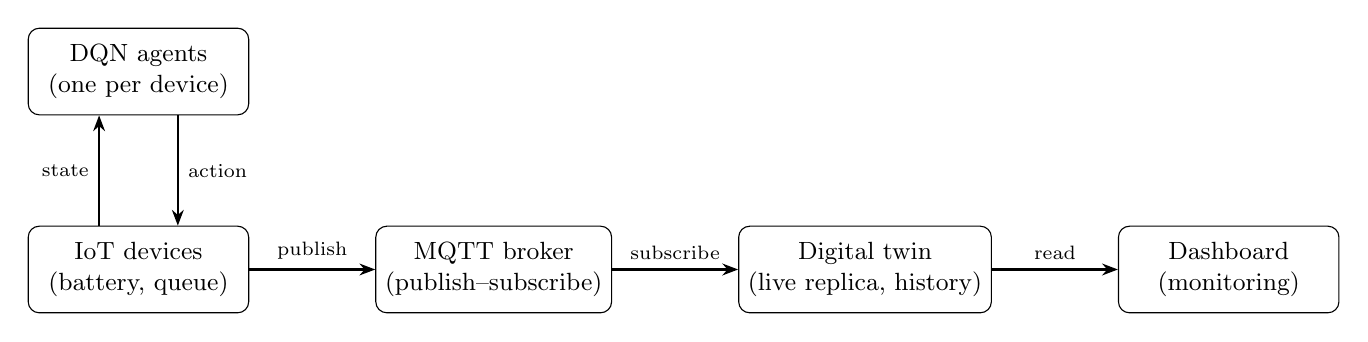
\begin{tikzpicture}[
  node distance=1.4cm and 1.6cm,
  box/.style={draw, rounded corners, align=center, minimum height=1.1cm, minimum width=2.8cm, font=\small},
  arr/.style={-{Stealth[length=2mm]}, thick}
]
\node[box] (dev) {IoT devices\\(battery, queue)};
\node[box, above=of dev] (agent) {DQN agents\\(one per device)};
\node[box, right=of dev] (mqtt) {MQTT broker\\(publish--subscribe)};
\node[box, right=of mqtt] (twin) {Digital twin\\(live replica, history)};
\node[box, right=of twin] (dash) {Dashboard\\(monitoring)};

\draw[arr] ([xshift=-0.5cm]dev.north) -- node[left,font=\scriptsize]{state} ([xshift=-0.5cm]agent.south);
\draw[arr] ([xshift=0.5cm]agent.south) -- node[right,font=\scriptsize]{action} ([xshift=0.5cm]dev.north);
\draw[arr] (dev) -- node[above,font=\scriptsize]{publish} (mqtt);
\draw[arr] (mqtt) -- node[above,font=\scriptsize]{subscribe} (twin);
\draw[arr] (twin) -- node[above,font=\scriptsize]{read} (dash);
\end{tikzpicture}
\caption{Overall architecture. Each IoT device is controlled by its own DQN agent. Device states are published over MQTT, and the digital twin subscribes to them and keeps a live replica that the dashboard reads.}
\label{fig:arch}
\end{figure*}

\subsection{IoT Device Layer}
Each device $i$ has a battery level $b_i \in [0,100]$ (in percent), a queue $q_i$ of pending data packets, and an alive flag. At every time step the device executes one of two actions: \emph{sleep} or \emph{send}. Sending consumes more energy than sleeping and removes one packet from the queue if the queue is not empty. A device whose battery reaches zero is marked as dead and receives a large penalty. In the simulated environment, a new packet arrives in the queue with probability $0.3$ at every step, and the initial queue length is drawn uniformly from $\{0,\dots,5\}$. The energy cost of an action can also be driven by real consumption data, as described in Section~\ref{sec:setup}.

\subsection{Agent Layer}
Every device has its own DQN agent with its own network weights and replay memory. Agent $i$ observes only the state $(b_i, q_i)$ of its own device and chooses the action for that device. Agents do not share parameters, observations, or experience, so no communication between devices is required for decision making.

\subsection{Digital Twin Layer}
The digital twin consists of one twin object per device. Each twin stores the latest reported state of its device, the time of the last update, and a bounded history of the 100 most recent states. A manager object holds all twins and updates the corresponding twin whenever a new state arrives. A Streamlit dashboard reads the twin, instead of querying the devices, to display the live device states and the learning curves.

\subsection{MQTT Synchronization}
Synchronization uses the publish--subscribe protocol MQTT \cite{mqtt}. Each device publishes its state as a JSON message containing the battery level, queue length, and alive flag to a per-device topic. The twin side subscribes to the topics of all devices using a single-level wildcard and updates the matching twin on every message. In the prototype, a public test MQTT broker is used with the default quality-of-service level. This decouples the devices from the twin, so that they can run on different machines.

\subsection{Prototype Scope}
The results of Section~\ref{sec:results} were produced without the twin, which only mirrors the device states and does not influence the agents. In the training scripts and the dashboard the twin is updated in-process after every step, and the MQTT pipeline was evaluated separately (Section~\ref{sec:mqtt}). The information flow is one-directional, from the devices to the twin.

\section{Problem Formulation and Learning Method}
\label{sec:method}

\subsection{Per-Device Decision Problem}
Each device $i$ is modeled as a Markov decision process. At time step $t$ the state is $s_{i,t}=(b_{i,t}, q_{i,t})$, where $b_{i,t}\in[0,100]$ is the battery level in percent and $q_{i,t}\in\mathbb{N}_0$ is the number of pending data packets. The action $a_{i,t}\in\{0,1\}$ is \emph{sleep} ($0$) or \emph{send} ($1$). The agent therefore sees only the local state of its own device. The dynamics of different devices are independent of each other in our environments, so each agent faces a stationary single-agent problem, which is the setting in which independent learning is well founded.

\textbf{Battery dynamics.} The battery decreases by an action-dependent cost $c(a_{i,t})$:
\begin{equation}
b_{i,t+1} = \max\bigl(0,\; b_{i,t} - c(a_{i,t})\bigr).
\end{equation}
In the simulated environment, $c(1)=2.0$ and $c(0)=0.2$. In the real-data environment the cost follows the recorded energy consumption $e_i(t)$ of household $i$:
\begin{equation}
c(1) = \kappa_i\, e_i(t), \qquad c(0) = 0.1\,\kappa_i\, e_i(t), \qquad \kappa_i = \frac{2.0}{\bar{e}_i},
\end{equation}
where $\bar{e}_i$ is the mean of the readings of household $i$. The scaling factor $\kappa_i$ makes an average reading cost about $2\%$ of the battery when sending, and sleeping reduces the cost to $10\%$ of that value. The reading index advances by one at every step and wraps around at the end of the series. At the start of each episode, the index is drawn uniformly at random from the series of the household.

\textbf{Queue dynamics.} Sending removes one packet if $q_{i,t}>0$. After the action, a new packet arrives with probability $0.3$:
\begin{equation}
q_{i,t+1} = q_{i,t} - \mathbf{1}[a_{i,t}=1,\, q_{i,t}>0] + \xi_{i,t},
\end{equation}
where $\xi_{i,t}\sim\text{Bernoulli}(0.3)$.

\textbf{Reward.} The reward encourages sending when data is waiting, sleeping when nothing is pending, and avoiding both a growing queue and battery depletion:
\begin{equation}
r_{i,t} =
\begin{cases}
1 + 0.3\,(q_{i,t}-1), & a_{i,t}{=}1,\; q_{i,t}{>}0,\\
-1, & a_{i,t}{=}1,\; q_{i,t}{=}0,\\
+0.5, & a_{i,t}{=}0,\; q_{i,t}{=}0,\\
+0.1, & a_{i,t}{=}0,\; q_{i,t}\in\{1,2\},\\
-0.5\,q_{i,t}, & a_{i,t}{=}0,\; q_{i,t}\ge 3,
\end{cases}
\end{equation}
and an additional penalty of $-10$ is applied in the step in which the battery reaches zero, after which the device is marked dead and receives zero reward. The first case grows with the remaining queue, so clearing a longer backlog is rewarded more.

\subsection{Deep Q-Network Agent}
Each agent approximates the action-value function $Q(s,a;\theta)$ with a fully connected network with one hidden layer of 16 ReLU units and two linear outputs, one per action. The input is the normalized state $\tilde{s}=(b/100,\; q/10)$, which puts both inputs on a similar scale. The agent selects actions $\epsilon$-greedily: with probability $\epsilon$ it picks a random action, otherwise $a=\arg\max_{a'}Q(s,a';\theta)$.

Transitions $(s,a,r,s',d)$, where $d$ indicates that the device died, are stored in a replay memory. For a transition sampled from the memory, the learning target is
\begin{equation}
y =
\begin{cases}
r, & d=1,\\
r + \gamma \max_{a'} Q(s',a';\theta^{-}), & d=0,
\end{cases}
\end{equation}
where $\theta^{-}$ are the parameters of a target network that is a periodic copy of $\theta$, which stabilizes learning \cite{mnih2015}. The parameters are updated by a gradient step on the squared error $\tfrac{1}{2}\bigl(Q(s,a;\theta)-y\bigr)^2$, with each gradient component clipped to $[-5,5]$ to prevent numerical divergence. The networks, backpropagation, and replay memory are implemented directly in NumPy.

\subsection{Training Procedure}
Training proceeds in episodes. At the start of an episode, every device is reset to a full battery and a random initial queue in $\{0,\dots,5\}$. In every step, each agent chooses an action for its own device, the environment returns the rewards and next states, the transitions are stored, and every agent performs one learning update. An episode lasts 30 steps and ends early only if all devices die. After every update, $\epsilon$ is multiplied by a decay factor until it reaches its minimum value. The hyperparameters are listed in Table~\ref{tab:hyper}.

\begin{table}[t]
\caption{DQN hyperparameters}
\label{tab:hyper}
\centering
\small
\begin{tabular}{@{}ll@{}}
\toprule
Parameter & Value \\
\midrule
Hidden layer & 16 units, ReLU \\
Discount factor $\gamma$ & 0.95 \\
Learning rate (SGD) & 0.0007 \\
Replay memory size & 5000 \\
Batch size per update & 16 \\
$\epsilon$ (start / min / decay) & 1.0 / 0.05 / 0.995 \\
Target network update & every 25 updates \\
Gradient clipping & $\pm 5$ per component \\
Episodes / steps per episode & 300 / 30 \\
\bottomrule
\end{tabular}
\end{table}

\section{Experimental Setup}
\label{sec:setup}

\subsection{Environments}
Two environments are used. Both contain $N$ devices, each described by the state, action, and reward definitions of Section~\ref{sec:method}.

\textbf{Simulated environment.} This environment has $N=3$ devices. Sending costs $2.0$ and sleeping costs $0.2$ percentage points of battery per step, and a new packet arrives with probability $0.3$ at each step.

\textbf{Real-data environment.} This environment has $N=5$ devices, one per household in the dataset described below. The battery cost of each step follows the recorded energy consumption of the household, scaled as in Section~\ref{sec:method}. The queue dynamics are the same as in the simulated environment, so the packet arrivals remain synthetic and only the energy cost is data-driven. At the start of every episode, each device begins at a random position of the consumption series of its household, so that training and evaluation cover the whole dataset.

In both environments, every episode lasts 30 steps and starts with a full battery and a random initial queue in $\{0,\dots,5\}$.

\subsection{Dataset}
The real-data environment uses the London Smart Meters dataset \cite{lcl2015}, released by UK Power Networks from the Low Carbon London project under a CC BY 4.0 licence. It contains half-hourly electricity consumption (kWh per half hour) of 5,567 London households between 2011 and 2014. We use one file of the public release (\texttt{LCL-June2015v2\_0.csv}) and select the first five households that have 1000 consecutive half-hourly readings (about 21 days) without gaps or missing values; each step of the environment corresponds to one reading. Only the consumption column is used. The mean consumption of the selected households ranges from 0.03 to 0.44 kWh per half hour, and the readings are bursty: the largest reading of a household is 7 to 12 times its mean. After the scaling of Section~\ref{sec:method}, a single reading can therefore cost up to about 23\% of the battery when sending.

\subsection{Baselines}
The trained agents are compared with four baselines. \emph{Random} chooses sleep or send with equal probability. \emph{Always-send} and \emph{Always-sleep} always choose the same action. \emph{Queue-threshold} is a hand-designed rule that sends whenever the queue is not empty and sleeps otherwise; it uses the queue length but not the battery level.

\subsection{Evaluation Protocol}
For each of 10 random seeds, the agents are trained for 300 episodes of 30 steps. They are then evaluated for 30 episodes with $\epsilon=0$ and no learning. Every policy is evaluated on the same 30 episodes, i.e., with the same initial queues, start positions, and packet arrivals, in both the simulated and the real-data environment. We report the mean and standard deviation of the per-seed averages. Because all seeds share the same evaluation episodes, the fixed policies (always-send, always-sleep, queue-threshold) have zero variance across seeds; only the learned and random policies vary. All results can be reproduced with the script \texttt{experiments.py} and \texttt{prepare\_dataset.py} distributed with the code.

\subsection{Metrics}
Let $T$ be the number of steps of an episode. We report four metrics, each averaged over the evaluation episodes:
\begin{itemize}
    \item the mean remaining battery at the end of the episode, $\bar{b}=\frac{1}{N}\sum_{i} b_{i,T}$, in percent, where higher is better;
    \item the mean number of pending packets at the end of the episode, $\bar{q}=\frac{1}{N}\sum_{i} q_{i,T}$ (the ``Queue'' column of the tables), where lower is better;
    \item the episode return, $G=\sum_{t}\sum_{i} r_{i,t}$, i.e., the sum of rewards over all devices and steps;
    \item the percentage of devices that are still alive at the end of the episode, where higher is better. Dead devices count with a battery of zero in $\bar{b}$.
\end{itemize}
The relative battery improvement over the random policy is $(\bar{b}_{\text{RL}}-\bar{b}_{\text{rand}})/\bar{b}_{\text{rand}}\times 100\%$.

\subsection{Implementation}
The environments, agents, and twin are implemented in Python with NumPy and pandas, MQTT uses the Paho client library, and the dashboard uses Streamlit. All experiments ran on a Linux machine with two Intel Xeon vCPUs (2.1~GHz) and 7~GB of RAM, without a GPU; the 10 seeds in both environments took about 10 minutes in total.

\section{Results and Discussion}
\label{sec:results}

\subsection{Training Behavior}
Fig.~\ref{fig:training} shows the episode return and the mean final battery level during training, averaged over 10 seeds. In both environments the return rises sharply during the first $\approx$50 episodes and then stays on a plateau, so the agents reach a stable policy quickly. The battery curve of the real-data environment is noisier because every episode starts at a random position of the consumption series. In the first 10--20 episodes there is a short transient in which the battery drops to about 50\% before it recovers to about 75\%.

\begin{figure*}[t]
\centering
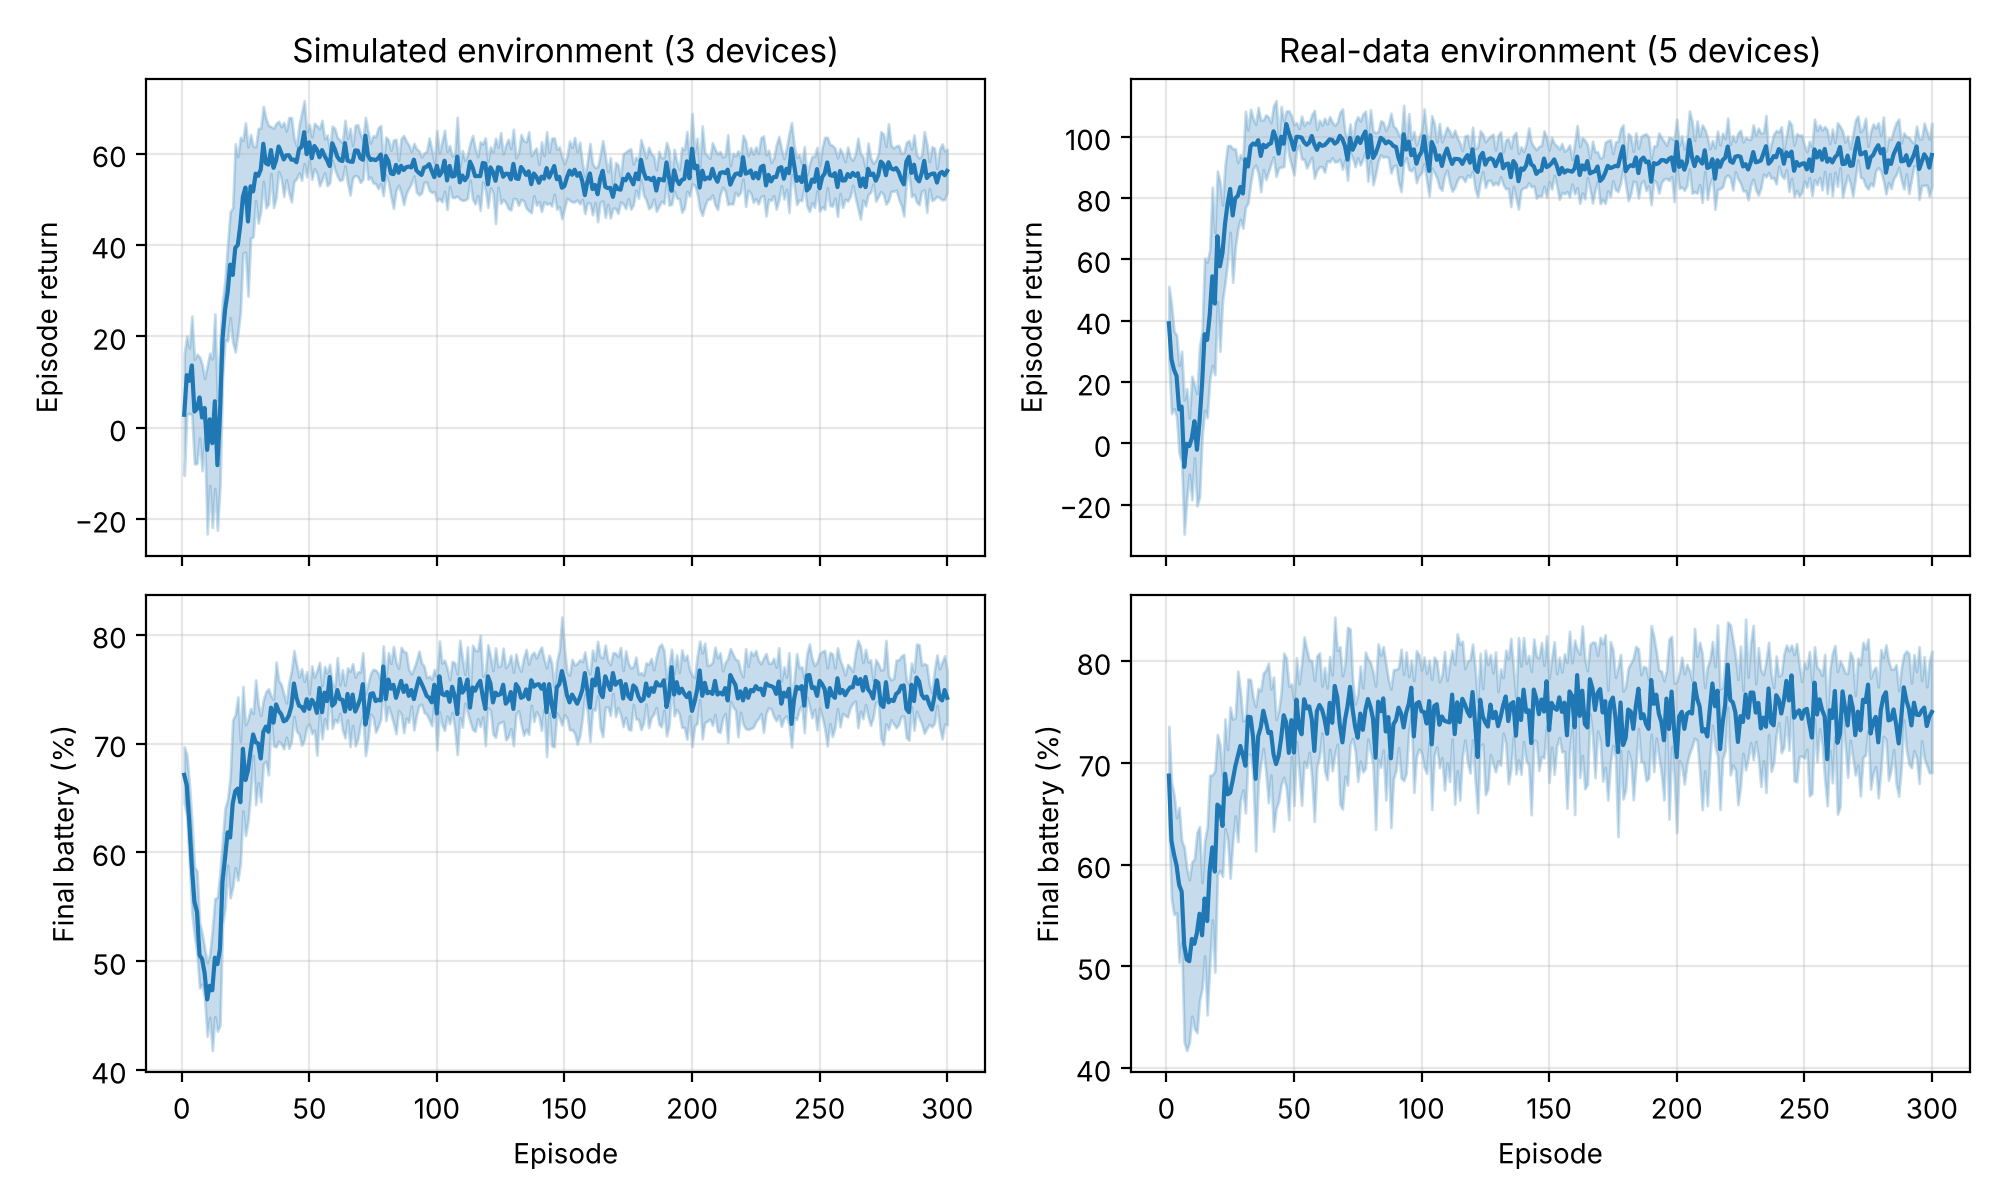
\includegraphics[width=0.85\textwidth]{fig_training.png}
\caption{Training curves (mean $\pm$ std over 10 seeds). Top: episode return. Bottom: mean battery level at the end of the episode. Left: simulated environment. Right: real-data environment.}
\label{fig:training}
\end{figure*}

\subsection{Comparison with Baselines}
Tables~\ref{tab:simulated} and~\ref{tab:real} compare the trained agents with the baselines after training, using greedy action selection on the same evaluation episodes for every policy.

\begin{table}[t]
\caption{Simulated environment (3 devices). Mean $\pm$ std over 10 seeds.}
\label{tab:simulated}
\centering\small
\footnotesize
\setlength{\tabcolsep}{2.5pt}
\begin{tabular}{@{}lcccc@{}}
\toprule
Policy & Battery (\%) & Queue & Return & Alive (\%) \\
\midrule
DQN (ours) & 75.2 $\pm$ 0.3 & 1.13 $\pm$ 0.17 & 56.7 $\pm$ 3.1 & 100 $\pm$ 0.0 \\
Random & 67.0 $\pm$ 0.7 & 1.06 $\pm$ 0.13 & 17.5 $\pm$ 3.2 & 100 $\pm$ 0.0 \\
Always-send & 40.0 $\pm$ 0.0 & 0.28 $\pm$ 0.00 & $-$20.2 $\pm$ 0.0 & 100 $\pm$ 0.0 \\
Always-sleep & 94.0 $\pm$ 0.0 & 11.34 $\pm$ 0.00 & $-$293.3 $\pm$ 0.0 & 100 $\pm$ 0.0 \\
Queue-threshold & 74.1 $\pm$ 0.0 & 0.28 $\pm$ 0.00 & 65.0 $\pm$ 0.0 & 100 $\pm$ 0.0 \\
\bottomrule
\end{tabular}
\end{table}

\begin{table}[t]
\caption{Real-data environment (5 devices). Mean $\pm$ std over 10 seeds.}
\label{tab:real}
\centering\small
\footnotesize
\setlength{\tabcolsep}{2.5pt}
\begin{tabular}{@{}lcccc@{}}
\toprule
Policy & Battery (\%) & Queue & Return & Alive (\%) \\
\midrule
DQN (ours) & 75.6 $\pm$ 0.4 & 1.05 $\pm$ 0.20 & 91.9 $\pm$ 6.8 & 99.5 $\pm$ 0.3 \\
Random & 66.1 $\pm$ 0.3 & 1.15 $\pm$ 0.07 & 26.6 $\pm$ 4.4 & 99.1 $\pm$ 0.5 \\
Always-send & 40.6 $\pm$ 0.0 & 0.29 $\pm$ 0.00 & $-$33.3 $\pm$ 0.0 & 92.0 $\pm$ 0.0 \\
Always-sleep & 93.9 $\pm$ 0.0 & 11.55 $\pm$ 0.00 & $-$508.7 $\pm$ 0.0 & 100 $\pm$ 0.0 \\
Queue-threshold & 73.4 $\pm$ 0.0 & 0.31 $\pm$ 0.00 & 109.5 $\pm$ 0.0 & 99.3 $\pm$ 0.0 \\
\bottomrule
\end{tabular}
\end{table}

\textbf{Comparison with the random policy.} The trained agents end the episode with 75.2\% (simulated) and 75.6\% (real-data) of their battery, compared with 67.0\% and 66.1\% for the random policy. This is a relative improvement of 12.2\% and 14.3\%, obtained at a comparable pending queue (1.13 vs.\ 1.06 and 1.05 vs.\ 1.15 packets per device). The return is more than three times higher (56.7 vs.\ 17.5 and 91.9 vs.\ 26.6). In the real-data environment, the share of devices alive at the end of the episode is comparable (99.5\% vs.\ 99.1\%).

\textbf{The two objectives conflict.} Always-send keeps the queue small (0.28 and 0.29 packets per device) but ends with only about 40\% battery and, in the real-data environment, loses 8\% of the devices, because bursts of high consumption deplete the battery. Always-sleep ends with about 94\% battery but leaves 11.3 to 11.6 packets pending per device. Battery alone is therefore not a sufficient metric, and a useful policy must balance both.

\textbf{Comparison with the queue-threshold heuristic.} The hand-designed Queue-threshold policy, which sends whenever the queue is not empty, achieves the highest return in both environments (65.0 and 109.5). The return of the DQN agents (56.7 and 91.9) is about 13\% and 16\% lower, and the heuristic keeps the queue much shorter (0.28 and 0.31 vs.\ 1.13 and 1.05). The DQN agents retain about 1.1 and 2.2 percentage points more battery than this heuristic but leave about 0.7 to 0.9 more packets pending per device. The share of surviving devices is the same within the variation between seeds (99.5\% vs.\ 99.3\%). Under the reward used here, the learned policy is therefore clearly better than the random, always-send, and always-sleep policies, but it does not surpass the heuristic.

\subsection{MQTT Synchronization}
\label{sec:mqtt}
We measured the synchronization between devices and the twin separately from the learning experiments. A publisher emitted the states of 5 devices for 200 steps (one message per device every 0.1~s, 1000 messages in total) to the public HiveMQ broker (\texttt{broker.hivemq.com}) with the default quality-of-service level 0, using a private random topic. A subscriber with a single-level wildcard updated the twin objects of the devices. We define the delay as the time from the call to the publish function until the corresponding twin object has been updated, and the loss as the share of published states that never reached the twin. Publisher and subscriber ran in one process on one machine, so the same clock is used for both timestamps.

All 1000 messages reached the twin (0\% loss). The delay had a mean of 561~ms and a median of 291~ms, with a heavy tail: the 95th percentile was 2168~ms and the maximum 3175~ms. These values are dominated by the round trip over the internet to a shared public broker and are small compared with the 30-minute interval between the readings of the dataset used in the real-data environment. They come from a single run, and the delay will depend on the network, the broker, and the load.


\subsection{Discussion and Limitations}
In the 30-step episodes used here, the battery rarely limits behavior. In the simulated environment no device exhausts its battery (even always-send ends at 40\%), and in the real-data environment only the always-send policy loses a noticeable share of devices (8\%), while at most 1\% of the devices die under the other policies. The penalty for a dead device is therefore rarely triggered, the reward depends almost only on the action and the queue, and a queue-based rule is close to optimal. The agents recover an approximation of this rule from the reward alone, without being told that the queue matters, but the results do not show that reinforcement learning outperforms hand-crafted rules in this setting. A longer horizon in which the battery limits behavior is needed to test whether a battery-aware learned policy can beat queue-based rules.

Further limitations are as follows. The agents are independent and the devices do not interact, so the multi-agent structure is a decomposition of the problem rather than a coordination mechanism. Packet arrivals are synthetic, and only the energy cost in the real-data environment follows measured data, from a small dataset of five households. The MQTT measurement is a single run with a public broker and QoS 0, with publisher and subscriber on the same machine. The agents use a small network implemented in NumPy, and no other learning algorithm was compared.

\section{Conclusion and Future Work}
\label{sec:conclusion}

This paper presented a framework for energy-aware IoT management in which every device is controlled by its own DQN agent and mirrored by a digital twin synchronized over MQTT. The framework was evaluated in a simulated environment and in an environment driven by real household energy-consumption readings, over 10 random seeds. The trained agents retained about 12--14\% more battery than a random policy at a comparable pending queue, and clearly outperformed the always-send and always-sleep policies. A simple queue-threshold rule achieved a higher return than the learned agents, because in the short episodes the battery rarely limits the behavior. The results therefore show that lightweight per-device agents can learn a sensible transmit-or-sleep policy from the reward alone, but they do not show an advantage over hand-crafted rules in this setting.

Future work will use longer episodes in which batteries can be exhausted, so that the energy--latency trade-off becomes binding and battery-aware policies can be compared with queue-based rules using network lifetime as a metric. A shared wireless channel with collisions would create real interaction between devices and justify coordinated multi-agent learning. The digital twin will be placed in the decision loop, and the MQTT synchronization will be measured with higher quality-of-service levels, a private broker, and many more devices. Finally, stronger learning algorithms and larger real datasets will be evaluated.

\begin{thebibliography}{00}

\bibitem{zanella2014} A. Zanella, N. Bui, A. Castellani, L. Vangelista, and M. Zorzi, ``Internet of Things for smart cities,'' \emph{IEEE Internet Things J.}, vol. 1, pp. 22--32, 2014.

\bibitem{mnih2015} V. Mnih \emph{et al.}, ``Human-level control through deep reinforcement learning,'' \emph{Nature}, vol. 518, no. 7540, pp. 529--533, 2015.

\bibitem{grieves2017} M. Grieves and J. Vickers, ``Digital twin: Mitigating unpredictable, undesirable emergent behavior in complex systems,'' in \emph{Transdisciplinary Perspectives on Complex Systems}. Springer, 2017, pp. 85--113.

\bibitem{mqtt} OASIS, ``MQTT Version 5.0,'' OASIS Standard, Mar. 2019.

\bibitem{ye2002smac} W. Ye, J. Heidemann, and D. Estrin, ``An energy-efficient MAC protocol for wireless sensor networks,'' in \emph{Proc. IEEE INFOCOM}, 2002, pp. 1567--1576.

\bibitem{luong2019} N. C. Luong \emph{et al.}, ``Applications of deep reinforcement learning in communications and networking: A survey,'' \emph{IEEE Commun. Surveys Tuts.}, vol. 21, no. 4, pp. 3133--3174, 2019.

\bibitem{chu2019} M. Chu, H. Li, X. Liao, and S. Cui, ``Reinforcement learning-based multiaccess control and battery prediction with energy harvesting in IoT systems,'' \emph{IEEE Internet Things J.}, vol. 6, no. 2, pp. 2009--2020, Apr. 2019.

\bibitem{zhang2021marl} K. Zhang, Z. Yang, and T. Ba\c{s}ar, ``Multi-agent reinforcement learning: A selective overview of theories and algorithms,'' in \emph{Handbook of Reinforcement Learning and Control}. Springer, 2021, pp. 321--384.

\bibitem{tan1993} M. Tan, ``Multi-agent reinforcement learning: Independent vs. cooperative agents,'' in \emph{Proc. ICML}, 1993, pp. 330--337.


\bibitem{fuller2020} A. Fuller, Z. Fan, C. Day, and C. Barlow, ``Digital twin: Enabling technologies, challenges and open research,'' \emph{IEEE Access}, vol. 8, pp. 108952--108971, 2020.

\bibitem{tao2019} F. Tao, H. Zhang, A. Liu, and A. Y. C. Nee, ``Digital twin in industry: State-of-the-art,'' \emph{IEEE Trans. Ind. Informat.}, vol. 15, no. 4, pp. 2405--2415, 2019.

\bibitem{lu2021} Y. Lu, S. Maharjan, and Y. Zhang, ``Adaptive edge association for wireless digital twin networks in 6G,'' \emph{IEEE Internet Things J.}, vol. 8, no. 22, pp. 16219--16230, 2021.

\bibitem{lcl2015} UK Power Networks, ``SmartMeter energy consumption data in London households,'' London Datastore, Low Carbon London project, CC BY 4.0. [Online]. Available: \url{https://data.london.gov.uk/dataset/smartmeter-energy-use-data-in-london-households}

\end{thebibliography}

\end{document}
